\section{Data Overview}
Schematically, the observation and action data that will be recorded has the following format. The observations consist of a 360 degree laser scan with ranges from 0.0 to 3.5 meters and the position of the goal in polar coordinates in the robot’s own coordinate frame. As can be seen in figure \ref{fig:observation-space-scan}, the robot is only aware of portions of objects that are contained within a 3.5m radius, such as the circular dynamic obstacle and wall shown. If at a given angle no object is within the 3.5m range, a value of 3.5 is recorded. As can be seen in figure \ref{fig:observation-space-goal}, the goal in the robot's coordinate frame is located at the transition of $\pi$ and $-\pi$ degrees.
%\myfig{observation_laser_scan_300.png}%% filename
% {width=0.6\textwidth}%% width/height
% {Schematic overview of the laser scan. The %range is 3.5m.}%% caption
% {Observation Space: Laser Scan}%% optional %(short) caption for list of figures
% {fig:observation-space-scan}%% label
% \FloatBarrier
% \myfig{observation_space_300.png}%% filename
% {width=0.6\textwidth}%% width/height
% {Schematic overview of the goal in the %robot's coordinate frame.}%% caption
% {Observation Space: Goal in robot frame}%% optional (short) caption for list of figures
% {fig:observation-space-goal}%% label
% \FloatBarrier
 
 The actions consist of a linear velocity ranging from 0.0 meters per second to 0.3 meters per second and an angular velocity ranging from -2.7 meters per second to 2.7 meters per second, see figure \ref{fig:action-space}.
  %\myfig{action_space_300.png}%% filename
 %{width=0.4\textwidth}%% width/height
 %{Schematic overview of the robot's action space, consisting of a linear velocity and an angular velocity.}%% caption
 %{Action Space}%% optional (short) caption for list of figures
 %{fig:action-space}%% label
 %\FloatBarrier
 

\begin{figure}
\centering
\begin{subfigure}[b]{0.4\textwidth}
   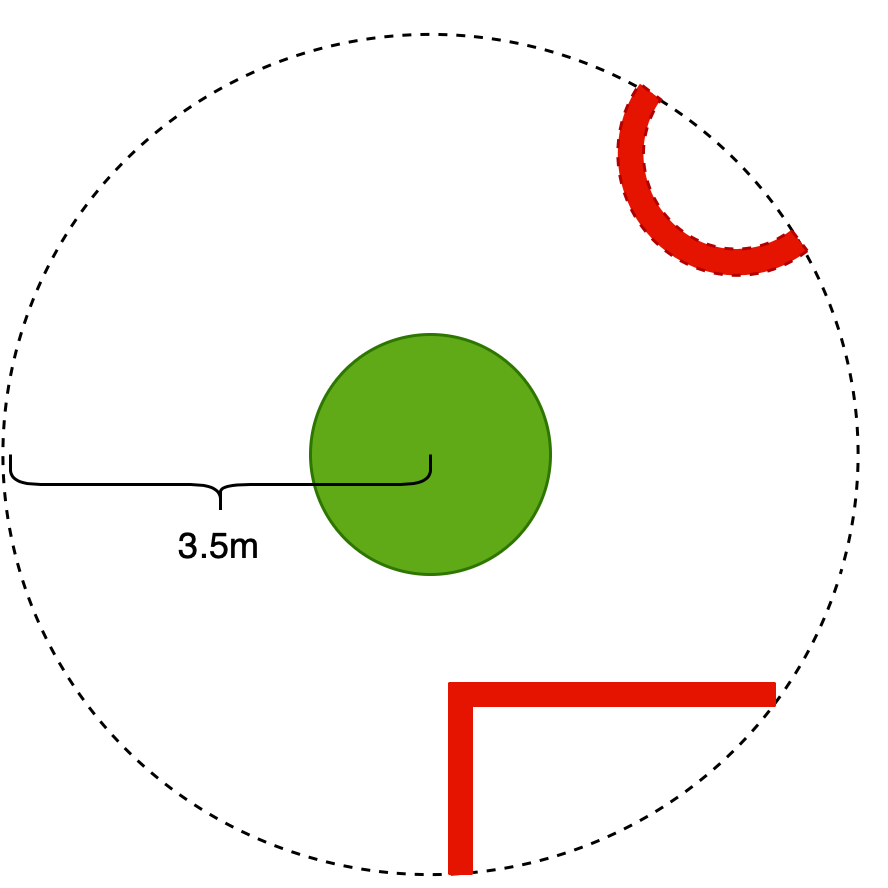
\includegraphics[width=1\linewidth]{figures/observation_laser_scan_300.png}
   \caption{Observation Space: Laser Scan}
   \label{fig:observation-space-scan} 
\end{subfigure}

\begin{subfigure}[b]{0.6\textwidth}
   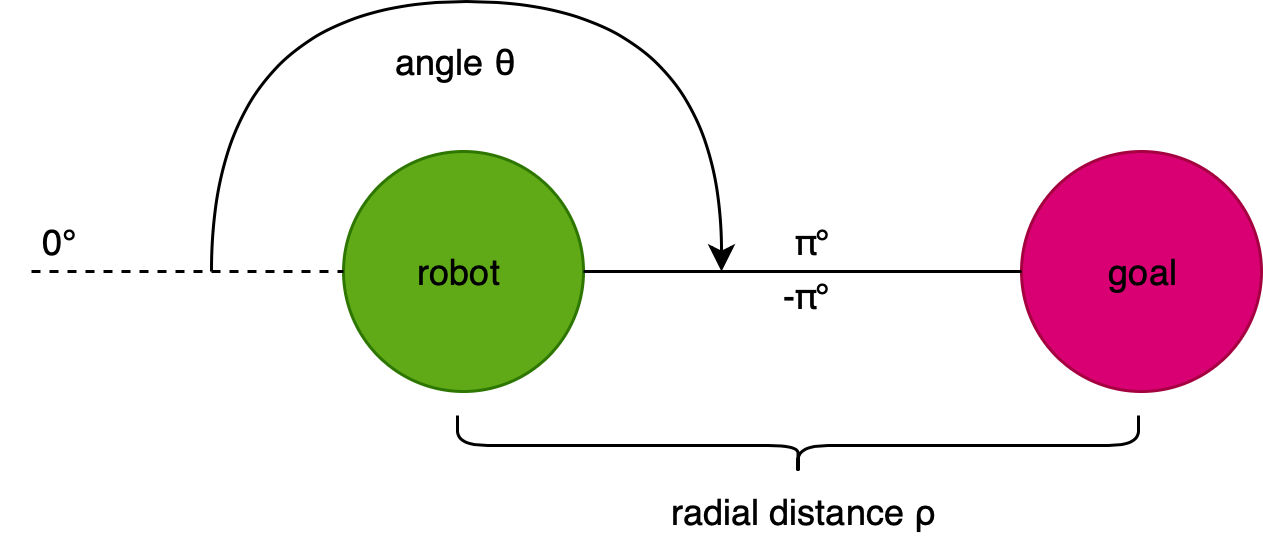
\includegraphics[width=1\linewidth]{figures/observation_space_300.png}
   \caption{Observation Space: Goal in Robot Frame}
   \label{fig:observation-space-goal}
\end{subfigure}
\begin{subfigure}[b]{0.4\textwidth}
   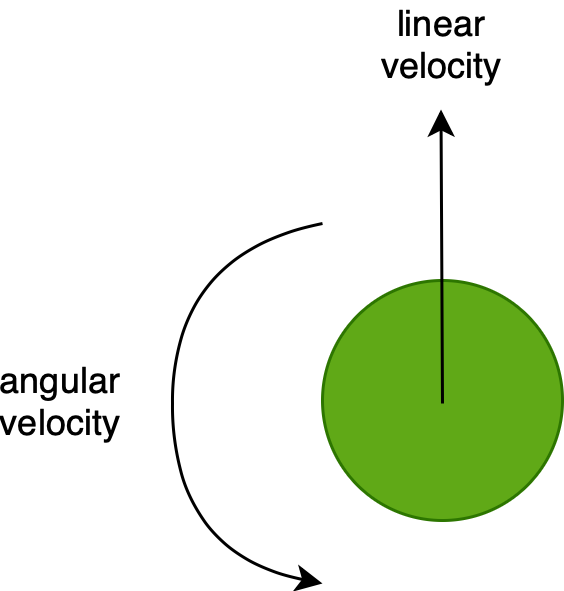
\includegraphics[width=1\linewidth]{figures/action_space_300.png}
   \caption{Action Space}
   \label{fig:action-space}
\end{subfigure}

\caption[]{Schematic overview of a) the laser scan (the range is 3.5m), b) the goal in the robot's coordinate frame, c) the robot's action space, consisting of a linear velocity and an angular velocity.}
\end{figure}